\documentclass{article}
\usepackage{graphicx}
\usepackage[english,greek]{babel}
\usepackage[utf8x]{inputenc}
\usepackage{amsmath}
\usepackage{relsize}
\usepackage{enumerate}
\usepackage[parfill]{parskip}
\usepackage{graphicx}
\usepackage{listings}

\makeatletter
\renewcommand*\env@matrix[1][*\c@MaxMatrixCols c]{%
  \hskip -\arraycolsep
  \let\@ifnextchar\new@ifnextchar
  \array{#1}}
\makeatother

\begin{document}

\title{\vspace{-3.5cm}\textbf{Τεχνικές Εξόρυξης Δεδομένων \\ \textlatin{Project \#}1}}
\author{Λάμπρου Ιωάννης \\1115201400088\\\\ Στεφανίδης - Βοζίκης Κωνσταντίνος \\1115201400192}

\maketitle
\section{\textlatin{WordCloud}}
Για την δημιουργία των \textlatin{wordclouds} κάθε κατηγορίας χρησιμοποιήθηκε το κείμενο από όλα τα άρθρα
που υπήρχαν στο \textlatin{train\_set.csv}. Τα \textlatin{wordclouds} που δημιουργήθηκαν ανά κατηγορία είναι: \\
\subsection*{\textlatin{Politics}}

\includegraphics[scale=0.6]{Poli}
\subsection*{\textlatin{Film}}
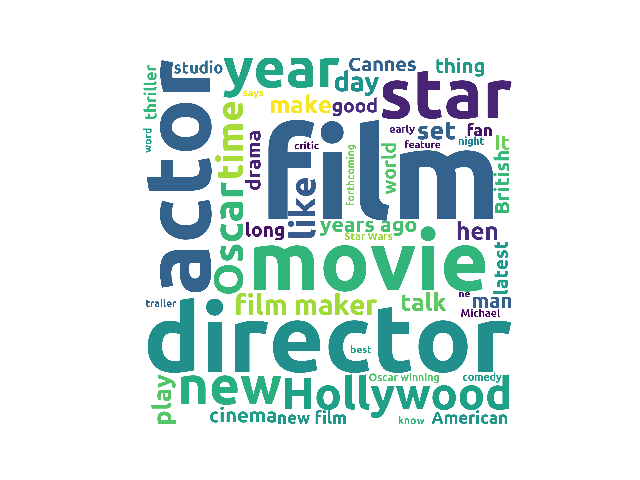
\includegraphics[scale=0.6]{Film}
\subsection*{\textlatin{Football}}
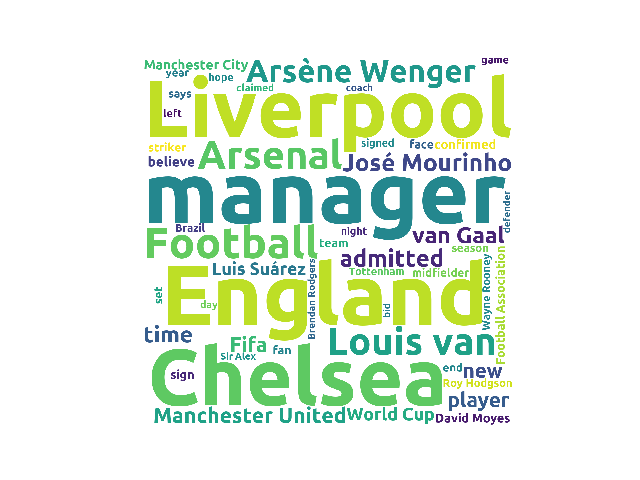
\includegraphics[scale=0.6]{Foot}
\subsection*{\textlatin{Business}}

\includegraphics[scale=0.6]{Busi}
\subsection*{\textlatin{Technology}}

\includegraphics[scale=0.6]{Techno}

Αξίζει να σημειωθεί πως για να δημιουργηθούν αυτά τα \textlatin{wordclouds}, θεωρήθηκαν ως \textlatin{stopwords} 
τα \textlatin{english stopwords} της βιβλιοθήκης \textlatin{sklearn}
στις οποίες προστέθηκαν οι λέξεις \textlatin{'say', 'said', 'th', 'it,} και \textlatin{'ha'}, τις οποίες κρίναμε ως επιπλέον 
\textlatin{stopwords}, μετά από εμφάνισή τους στα \textlatin{wordclouds} αυτά. 

\section{Υλοποίηση Κατηγοριοποίησης \textlatin{(Classification)}}
Για την κατηγοριοποίηση δοκιμάστηκαν όλες οι ζητούμενες μέθοδοι κατηγοριοποίησης, δηλαδή οι 
\textlatin{Support Vector Machines (SVM), Random Forests, Multinomial Naive Bayes}, καθώς και 
έγινε δική μας υλοποίηση της μεθόδου \textlatin{K-Nearest Neighbors}.\\\\
Ακόμα, για την αξιολόγηση της απόδοσης όλων αυτών των μεθόδων χρησιμοποιήθηκε
\textlatin{10-fold Cross Validation} για όλες τις ζητούμενες μετρικές της εκφώνησης
\textlatin{(Precision, Recall, F-Measure, Accuracy)} που παρέχει η βιβλιοθήκη \textlatin{scikit}.\\
Όπως ζητήθηκε, για την προεπεξεργασία των δεδομένων χρησιμοποιήθηκε η τεχνική 
\textlatin{Latent Semantic Indexing (LSI)}. Κρατώντας τους παραπάνω \textlatin{classifiers} 
(\textlatin{SVM, Random Forests, Multinomial Naive Bayes, KNN}) συν τον βέλτιστο αλγόριθμο \textlatin{SVM} 
που επιλέξαμε σταθερούς, με το 
\textlatin{component number} να παίρνει τιμές 50,100,200, και με \textlatin{10-fold Cross Validation}
παίρνουμε τις τιμές για \textlatin{Accuracy}:\\\\

\renewcommand{\arraystretch}{2.5}
\begin{tabular}{ c c|c|c|}
\hline  
 Μέθοδοι & 50 & 100 & 200\\
\hline 
\textlatin{Multinomial Naive Bayes} & 0.9310288602641448 & 0.9413011576716126	 & 0.9466818848850481\\
\hline 
\textlatin{Random Forests} & 0.9157019403228437 & 0.904695907386271 & 0.8894505136148704\\
\hline
\textlatin{Support Vector Machines} & 0.8835806293820316 & 0.8252078917332464 & 0.5443502364258928\\
\hline
\textlatin{K-Nearest Neighbors} & 0.904614831330411 & 0.9038795401455294 & 0.8915692460689411\\
\hline
\textlatin{Support Vector Machines} (βέλτιστο) & 0.9624979618457525 & 0.9660851133213761 & 0.9656774824718735\\
\hline\\
\end{tabular}

Όπως παρατηρούμε, σχεδόν σε όλους τους αλγορίθμους, ο αριθμός \textlatin{components} 100 είναι καλύτερος από 
50, εκτός από την περίπτωση του αλγορίθμου \textlatin{SVM} χωρίς παραμέτρους, του οποίου τα αποτελέσματα χειροτερεύουν
σημαντικά. 
Όσο όμως αυξάνουμε τον αριθμό των \textlatin{components} από 100 και μετά, παρατηρούμε γενικά μια πτώση στο 
\textlatin{Accuracy}.\\\\

Ακόμα, για το \textlatin{Classification}, η πληροφορία του τίτλου και η πληροφορία που παίρνουμε από το κείμενο
έχουν ίδιο βάρος, 50-50.\\\\

Επίσης, όπως προαναφέρθηκε, χρησιμοποιήθηκε δική μας υλοποίηση για την μέθοδο \textlatin{K-Nearest Neighbors},
\textlatin{(nearest\_neighbor\_validation()} η οποία καλεί την\\ \textlatin{find\_k\_nearest()} στον κώδικά μας)
ενώ και η τελική επιλογή για \textlatin{predicted label} έγινε με \textlatin{majority voting}.\\

Τέλος, στον κώδικά μας τρέχουμε την μέθοδο \textlatin{Support Vector Machines} χωρίς παραμέτρους, ή να δοκιμάσουμε
τυχαίες τιμές παραμέτρων, με το καλύτερο αποτέτεσμα να παραμένει χειρότερο από αυτό των 
\textlatin{Support Vector Machines} χωρίς παραμέτρους. Τελικά, για το τρίτο ερώτημα, βρήκαμε τις βέλτιστες παραμέτρους. 

\section{\textlatin{Beat the Benchmark}}
Για το ερώτημα αυτό βρήκαμε τις βέλτιστες παραμέτρους \textlatin{kernel='rbf', C=10, gamma=1} για τον αλγόριθμο \textlatin{Support Vector Machines} 
με τη χρήση της \textlatin{GridSearchCV()}. (μέσω της \textlatin{find\_parameters()} στον κώδικά μας). Η προσθήκη των παραμέτρων αυτών,
σε συνδυασμό με της εφαρμογής 100 \textlatin{component number} για το \textlatin{LSI}, βλέπουμε πως αποφέρει πολύ καλυτερα αποτελέσματα από όλους τους 
υπόλοιπους αλγορίθμους που έχουμε δοκιμάσει ως τώρα. 



\end{document}
